\documentclass[12pt]{article}
\usepackage{amsfonts,amssymb}
\usepackage{amsmath}
\usepackage{amsthm}
\usepackage{hyperref}
\usepackage{graphicx}
\usepackage{listings}
%\documentstyle[12pt,amsfonts]{article}
%\documentstyle{article}

\setlength{\topmargin}{-.5in}
\setlength{\oddsidemargin}{0 in}
\setlength{\evensidemargin}{0 in}
\setlength{\textwidth}{6.5truein}
\setlength{\textheight}{8.5truein}
%
%\input ../adgeomcs/lamacb.tex
%\input ../mac.tex
%\input ../mathmac.tex
%
\input xy
\xyoption{all}
\def\fseq#1#2{(#1_{#2})_{#2\geq 1}}
\def\fsseq#1#2#3{(#1_{#3(#2)})_{#2\geq 1}}
\def\qleq{\sqsubseteq}
\newtheorem{theorem}{Theorem}
%cis51109hw1

%
\begin{document}
\begin{center}
\fbox{{\Large\bf Graph Theory}}\\
\vspace{1cm}
\end{center}

\vspace{0.5cm}\noindent


\section*{What is a graph}

A graph $G$ is defined by a combination of a vertex set $V$ and an edge set $E \subseteq V \times V$.
It is common to see the notation

$G = (V,E)$

For example in the following graph

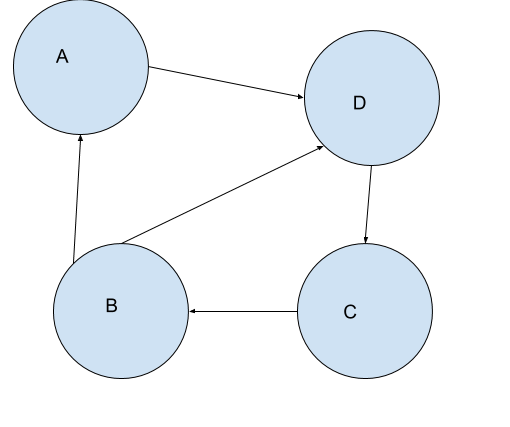
\includegraphics[scale=0.5]{./img/graph1.png}

We will mathematically write $G = (V, E)$ where 

$V = \{A,B,C,D\}$ and 

$E = \{(A,D), (D,C), (C,B), (B,A), (B,D)\}$

\section*{Terminology}

The two vertices that are part of an edge are its endpoints.

When a vertex is an endpoint of an edge we say the edge is incident on the vertex.

Note that two vertices connected by an edge is describing a relation (recall what that means from a previous part of the course).

A graph can either be directed meaning that there can be an edge from vertex $u$ to vertex $v$ without having an edge from vertex $v$ to vertex $u$ or undirected meaning that $(u,v) \in E \leftrightarrow (v,u) \in E$.

If we view this in terms of relations, an undirected graph is describing a symmetric relationship.

Loop(or sometimes self-loop) - an edge that joins a vertex to itself.

Complete graph - a graph where every vertex is connected to every other vertex.

A complete graph on $n$ vertices is denoted as $K_n$.

\medskip

\textbf{Question}

How many edges does a complete graph have?

\medskip

That is the same as $\binom{n}{2}$ since for any pair of distinct vertices they have to be connected by an edge.

\section*{Paths and walks}

For the remainder of the course we will be focusing on the following type of graph

\begin{itemize}
\item undirected
\item no self loops
\item no parallel edges
\item finite number of edges
\end{itemize}

whenever we have to deviate from this type of graph it will be made clear.


\textbf{Path} - A path is an alternating sequence of vertices and edges that satisfy the following 

\begin{enumerate}


\item it starts and ends with a vertex.
\item each edge joins the vertex before it in the sequence to the vertex after it in the sequence.
\item no vertex appears more than once.
\end{enumerate}

A \textbf{walk} satisfies the first two conditions but not the third

\medskip

\textbf{Result}

If there is a walk between two vertices $u$ and $v$, there has to be a path between vertices $u$ and $v$.

Proof

Consider any walk between vertices $u$ and $v$. There are two cases

Case 1 - There is no vertex that is repeated in the walk. In this case then by definition this walk is a path and we are done.

Case 2 - There exists a vertex $x$ in this walk such that it is repeated. For this vertex, we can make a shorter walk by removing the part of the walk that is between the first and last occurrences of the the vertex. That is, include the last occurrence of $x$ but not the first. Repeat the process of finding these repeated vertices and making shorter walks. Note that in each case we are eliminating one of the vertices from the list of repeated vertices. Therefore eventually we will have no repeated vertices in our walk and our walk will reduce to a path. (draw a picture to complete this proof).

\medskip

The length of a path is the number of edges in the path.

There can be multiple paths between two vertices. An algorithms course is likely to spend a fair number of lectures talking about different methods to find shortest paths in graphs.

\section*{Degrees}

The degree of a vertex is the number of edges that are incident on it. 

Note that if you have a self-loop, it counts twice to the degree of the vertex. We are allowing self loops in the discussion of degrees.

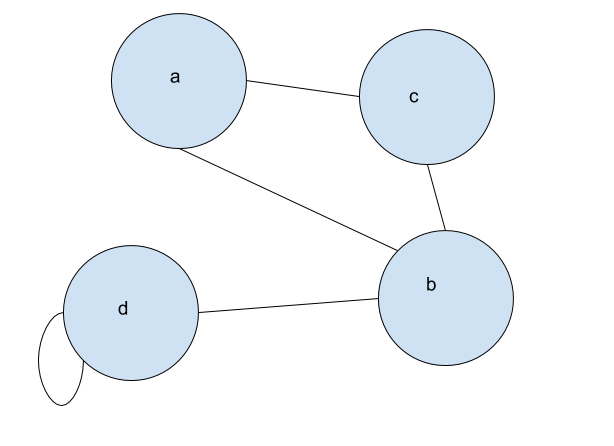
\includegraphics[scale=0.5]{./img/graph2.png}

In the above example the degree of vertex d, denoted by deg(d) = 3. deg(a) = 2 etc.

\begin{theorem}
Sum of the degrees of the vertices is twice the number of edges.
\end{theorem}

\textbf{Proof}

Proof by induction on the number of edges. Consider that we are given a graph with $e$ edges and we want to prove the result holds for any $e$.

Base case: If the number of edges is 0 then the sum of the degrees is 0. Twice the number of edges is also 0. Done.

Induction hypothesis: Suppose that for $0 < k \le e$  the result holds.

Now consider a graph with $e > 0$ edges. Let $e_1$ be some edge in this graph. Consider what happens when we delete this edge (note that deleting an edge means just deleting the edge and not deleting the associated vertices). We get a graph $G'$ which has 1 less edge. So we can apply the induction hypothesis to it.

Applying the induction hypothesis says that the sum of degrees of the vertices in $G'$ is $2(e-1)$.

Now let us consider 2 cases for the edge that we removed

Case 1: the removed edge was a self loop. When we add this edge back in the degree of one single vertex will go up by 2. So the sum of the degrees will be $2(e-1) + 2 = 2e$.

Case 2: the removed edge joined two distinct vertices. When we add this edge back the degree of two vertices goes up by 1 each. Again the sum of the degrees will be $2e$.


Combining this with the base case of 0 edges, we have a complete proof by induction. QED!

\section*{Using graphs to prove results}

A famous theorem says that in any group of 6 people you are bound to find either a group of 3 distinct mutual friends or 3 distinct mutual enemies (obviously this assumes for any given pair of people they are either mutual friends or mutual enemies). 

Proof

Consider one person. Call them Sally. Divide the rest of the people into 2 buckets - either they are friends of Sally's or enemies of Sally. Since we have 2 buckets and 5 people it must be the case that one of the buckets contains at least 3 people. Without loss of generality, let us assume the friends bucket has at least 3 people (if it has more than 3 it is even better for our proof).

Then let us draw the 'friendship' graph. It is going to look like this, with the red vertex being Sally.

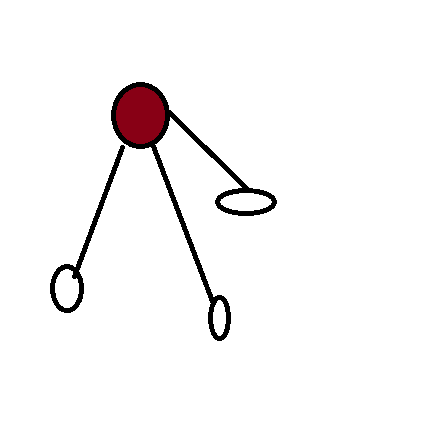
\includegraphics[scale=0.5]{./img/friends.png}

Now consider what happens if we add any edge to this graph. That would immediately create a triangle (a $K_3$) which means that we have 3 distinct mutual friends and we are done with proving the result.

Consider what happens if we do not add any edge to this graph. That would mean that none of Sally's friends are friends with each other. That immediately means that we have 3 enemies. 

So currently we have shown that if any person has 3 friends then the theorem is true. 

The remainder of the proof is simple because we only have to worry about  

a) what happens if an arbitrarily chosen person has more than 3 friends - this is easy because if that person has more than 3 friends we can pick any 3 of them and prove the result using the above argument.

b) what happens if the arbitrarily chosen person does not have at least 3 friends - this must mean that the chosen person has at least 3 enemies. That results in a similar argument to before with the words friend and enemy being interchanged.

\end{document}



